\documentclass{beamer}
\usepackage[utf8]{inputenc}
\usepackage{graphicx}
\usepackage{tikz}
\usetikzlibrary{shapes.geometric, arrows, positioning}

\usetheme{Madrid}
\usecolortheme{beaver}

% --- TikZ Style for Diagrams ---
\tikzstyle{block} = [rectangle, draw, fill=blue!20, text width=6em, text centered, rounded corners, minimum height=4em]
\tikzstyle{line} = [draw, -latex']
\tikzstyle{cloud} = [ellipse, draw, fill=orange!20, minimum height=4em, text width=5em, text centered]
\tikzstyle{user} = [circle, draw, fill=green!20, minimum size=1.5cm]

\title{Bachelor's Thesis Proposal: An MCP for Keylime}
\subtitle{Building an Intelligent Control Plane for Remote Attestation}
\author{Your Name / Department}
\institute{Your University}
\date{\today}

\begin{document}

\begin{frame}
  \titlepage
\end{frame}

\begin{frame}{Agenda}
  \tableofcontents
\end{frame}

\section{Introduction: The Problem}

\begin{frame}{The Challenge: Managing Trust at Scale}
    \begin{itemize}
        \item \textbf{Keylime} is a powerful tool for remote attestation, ensuring that our cloud and edge nodes are trustworthy.
        \vspace{1em}
        \item However, managing a large fleet of agents, policies, and their states can become a complex operational task.
        \vspace{1em}
        \item An administrator needs to manually query the Registrar and Verifier to understand the state of the system and take action.
        \vspace{1em}
        \item \textbf{The Question:} Can we create a more intelligent, conversational interface to manage Keylime's state and operations?
    \end{itemize}
\end{frame}

\section{Proposed Solution: The MCP Architecture}

\begin{frame}{What is an MCP?}
    \framesubtitle{Model Control Protocol}
    \begin{itemize}
        \item \textbf{MCP} is a design pattern for creating an intelligent, tool-based control plane for complex systems like Keylime.
        \vspace{1em}
        \item It separates the system's state from the actions that can be performed on it:
        \begin{itemize}
            \item \textbf{Model:} The current state of the system (e.g., all Keylime agents and their attestation status).
            \item \textbf{Control Protocol:} A defined set of "tools" or commands that can be used to query or modify the model.
        \end{itemize}
        \vspace{1em}
        \item \textbf{Our Thesis Idea:} We will build an MCP Server that implements this protocol for Keylime.
        \begin{itemize}
            \item The \textbf{MCP Server} exposes tools like \texttt{get\_agent\_status()}.
            \item A \textbf{Large Language Model (LLM)} acts as a smart client, translating natural language from an administrator into calls to this protocol.
        \end{itemize}
    \end{itemize}
\end{frame}

\begin{frame}{Proposed Architecture}
    \frametitle{An MCP Server for Keylime}
    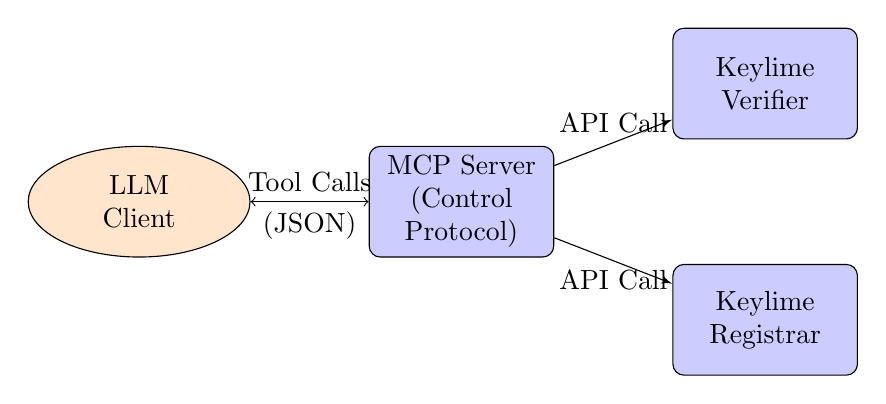
\begin{tikzpicture}[node distance=1.2cm and 1.5cm, auto]
        % Nodes
        \node [cloud] (llm) {LLM Client};
        \node [block, right=of llm] (mcp) {MCP Server (Control Protocol)};
        \node [block, right=of mcp, yshift=1.5cm] (verifier) {Keylime Verifier};
        \node [block, right=of mcp, yshift=-1.5cm] (registrar) {Keylime Registrar};

        % Arrows
        \path [line, <->] (llm) -- node[midway, above] {Tool Calls} node[midway, below] {(JSON)} (mcp);
        \path [line] (mcp) -- node[midway, above] {API Call} (verifier);
        \path [line] (mcp) -- node[midway, below] {API Call} (registrar);
    \end{tikzpicture}

    \begin{itemize}
        \item The \textbf{Administrator} asks questions in natural language.
        \item The \textbf{LLM Client} translates the question into a structured "Tool Call" defined by the Model Control Protocol.
        \item The \textbf{MCP Server} receives the call, executes the corresponding logic (querying the Keylime components), and returns a structured result.
        \item The LLM client uses this result to generate a human-readable answer for the administrator.
    \end{itemize}
\end{frame}

\section{Thesis Implementation Details}

\begin{frame}{The MCP Server: "Tools" as Functions}
    \framesubtitle{The server will be a simple web service (Python/Go)}

    The core of the thesis is to implement the "tools" the MCP server provides to the LLM. Each tool is a function that interacts with the Keylime backend.

    \begin{block}{Example Tools to Implement}
    \begin{itemize}
        \item \texttt{get\_all\_agents()}: Queries the Registrar for all registered agent UUIDs.
        \item \texttt{get\_agent\_status(agent\_uuid)}: Queries the Verifier for the attestation status of a specific agent.
        \item \texttt{get\_failed\_agents()}: Gets a list of all agents, queries the status of each, and returns only those that are in a "failed" state.
        \item \texttt{reactivate\_agent(agent\_uuid)}: Sends a command to the Verifier to reactivate a failed agent.
        \item \texttt{get\_agent\_policies(agent\_uuid)}: Fetches the IMA and TPM policies associated with an agent from the Verifier.
    \end{itemize}
    \end{block}
\end{frame}

\begin{frame}{The LLM Client: Perception and Action}
    \framesubtitle{Using LLM "Function Calling"}

    The student will use an LLM that supports "Function Calling" or "Tool Use" (like models from OpenAI, Google, or open-source models via Ollama/Podman AI Lab).

    \begin{enumerate}
        \item \textbf{Define the Tools:} You provide the LLM with a schema describing the available functions (e.g., "get\_agent\_status" and its parameters).
        \vspace{1em}
        \item \textbf{User Prompt:} The user asks: \textit{"What is the status of agent d432fbb3?"}
        \vspace{1em}
        \item \textbf{LLM Response:} The LLM doesn't answer directly. It returns a structured JSON object indicating which tool to call:
        \begin{center}
        \texttt{\{ "tool": "get\_agent\_status", "arguments": \{ "agent\_uuid": "d432fbb3" \} \}}
        \end{center}
        \vspace{1em}
        \item \textbf{Execution:} A client-side script executes the function by calling the MCP server, gets the result, and sends it back to the LLM.
        \vspace{1em}
        \item \textbf{Final Answer:} The LLM then generates a natural language response: \textit{"The status of agent d432fbb3 is 'pass'."}
    \end{enumerate}
\end{frame}

\section{Project Scope \& Evaluation}

\begin{frame}{Thesis Scope and Deliverables}
    \begin{itemize}
        \item \textbf{Deliverable 1: MCP Server Application.} A web service (e.g., using Python Flask/FastAPI or Go) that implements at least 5-7 core "tools" for interacting with the Keylime Registrar and Verifier.
        \vspace{1em}
        \item \textbf{Deliverable 2: LLM Client.} A command-line or simple web interface that allows a user to interact with the system in natural language. It will handle the communication loop with the LLM and the MCP server.
        \vspace{1em}
        \item \textbf{Deliverable 3: Documentation \& Testing.} Clear API documentation for the MCP server's tools and unit tests for each tool's functionality.
        \vspace{1em}
        \item \textbf{Evaluation:} The thesis will be evaluated on the correctness of the tool implementations, the robustness of the MCP server, and the effectiveness of the natural language interface in managing Keylime.
    \end{itemize}
\end{frame}

\end{document}
